\documentclass[12pt]{article}

% --- Packages ---
\usepackage[utf8]{inputenc}
\usepackage{geometry}
\usepackage{amsmath, amssymb}
\usepackage{hyperref}
\usepackage{graphicx} % Required for \includegraphics
\usepackage{fancyhdr}
\usepackage[dvipsnames]{xcolor}
\usepackage{enumitem}
\usepackage{autobreak}
\usepackage{breqn}
\usepackage{parskip}       % Correct paragraph spacing
\usepackage{xcolor}        % Required for \textcolor command
\usepackage{float}
\usepackage{listings}
\usepackage{tikz}
\usepackage[T1]{fontenc}
\usepackage{url}
\usepackage{amsthm}
\usepackage{booktabs}
\usepackage{pgfplotstable}
\usepackage{siunitx}
\usepackage{pgfplots}
\pgfplotsset{compat=1.18}

\usetikzlibrary{positioning, arrows.meta}
\setlist{nosep}           % Reduce vertical spacing in lists

% --- Page Setup ---
\geometry{a4paper, margin=1in, top=1.2in, headheight=35pt} % Expanded top margin & headheight for the ornament

\lstset{
    language=python,
    basicstyle=\ttfamily\small,
    backgroundcolor=\color{blue!5},
    keywordstyle=\color{purple!80!blue},
    commentstyle=\color{green!50!black},
    stringstyle=\color{red!70!black},
    numberstyle=\tiny\color{gray},
    numbers=left,
    numbersep=15pt,
    frame=shadowbox,
    rulesepcolor=\color{blue!20},
    frameround=tttt,
    breaklines=true,
    captionpos=b,
    showstringspaces=false,
    tabsize=4,
    xleftmargin=20pt,
    xrightmargin=5pt
}

% --- Header & Footer Configuration ---
\pagestyle{fancy}
\fancyhf{} % Clear default headers/footers

% Center the ornament in the header (antet)
\chead{
\includegraphics[width=4cm]{../ornament_6.pdf}}

% Center the page number in the footer
\cfoot{\thepage}

% Optional: Remove the default rule line below the header
\renewcommand{\headrulewidth}{0pt}

\begin{document}

\begin{titlepage}
	\thispagestyle{fancy} % Force header/footer onto the title page
	\centering

	\vspace*{4cm}

	% Main Title
	{\Huge \bfseries Homework 6}

	\vspace{4cm}

	% Name and Date
	{\Large \textbf{Name:} Gatman Vitalie} \\[0.5em]
	{\Large \textbf{Date:} \today} \\[0.5em]
	{\Large \textbf{Group:} FAF-263}

	\vfill
\end{titlepage}

\newpage

% Page 2 content...
\section*{Problem 6.1}
From the Handshaking Lemma, "The number of vertices of odd degree in a graph is always even."
We have a odd number of degres 3, however the number of verticies is 15 wich is even so is imposible to peer-to-peer network consists of 15 servers each being directly connected to exactly
3 other servers





\section*{6.2}
\[
	\begin{minipage}[t]{0.45\textwidth}
		\begin{align*}
			\varphi(v_6)                          & = w_1                            \\
			\varphi(v_5)                          & = w_2                            \\
			\varphi(v_1)                          & = w_3                            \\
			\varphi(v_2)                          & = w_4                            \\
			\varphi(v_7)                          & = w_5                            \\
			\textcolor{ForestGreen}{\varphi(w_6)} & \;\textcolor{ForestGreen}{= v_8} \\
			\textcolor{ForestGreen}{\varphi(w_7)} & \;\textcolor{ForestGreen}{= v_4} \\
			\varphi(v_3)                          & = w_8
		\end{align*}
	\end{minipage}%
	\begin{minipage}[t]{0.45\textwidth}
		\begin{align*}
			\varphi(w_1)                  & = v_6                    \\
			\varphi(w_2)                  & = v_5                    \\
			\varphi(w_3)                  & = v_1                    \\
			\varphi(w_4)                  & = v_2                    \\
			\varphi(w_5)                  & = v_7                    \\
			\textcolor{red}{\varphi(w_6)} & \;\textcolor{red}{= v_4} \\
			\textcolor{red}{\varphi(w_7)} & \;\textcolor{red}{= v_8} \\
			\varphi(w_8)                  & = v_3
		\end{align*}
	\end{minipage}
\]

\section*{Problem 6.3}
\begin{enumerate}[label=\alph*)]
	\item \noindent \\
	      \begin{minipage}[t]{0.58\textwidth}
		      \begin{center}
			      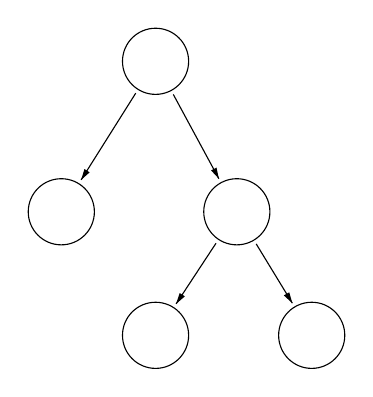
\begin{tikzpicture}[scale=0.3]
				      \draw (31.77, -4.65) circle (1.40);
				      \draw (27.78, -11.02) circle (1.40);
				      \draw (35.21, -11.02) circle (1.40);
				      \draw (31.77, -16.25) circle (1.40);
				      \draw (38.38, -16.25) circle (1.40);
				      \draw (30.93, -6.00) -- (28.62, -9.67);
				      \fill (28.76,-9.21) -- (28.98,-9.35) -- (28.62,-9.67) -- cycle;
				      \draw (32.52, -6.05) -- (34.45, -9.62);
				      \fill (34.12,-9.27) -- (34.35,-9.15) -- (34.45,-9.62) -- cycle;
				      \draw (34.33, -12.35) -- (32.64, -14.92);
				      \fill (32.79,-14.46) -- (33.01,-14.60) -- (32.64,-14.92) -- cycle;
				      \draw (36.03, -12.38) -- (37.56, -14.89);
				      \fill (37.20,-14.56) -- (37.43,-14.43) -- (37.56,-14.89) -- cycle;
			      \end{tikzpicture}
		      \end{center}
	      \end{minipage}%
	      \begin{minipage}[t]{0.45\textwidth}
		      \begin{center}
			      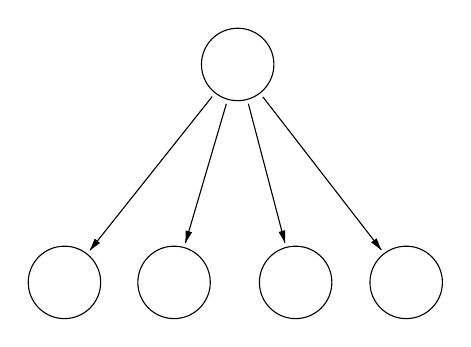
\begin{tikzpicture}[scale=0.4]
				      \draw (29.31, -1.53) circle (1.15);
				      \draw (23.81, -8.45) circle (1.15);
				      \draw (31.15, -8.45) circle (1.15);
				      \draw (34.66, -8.45) circle (1.15);
				      \draw (27.29, -8.45) circle (1.15);
				      \draw (28.50, -2.55) -- (24.62, -7.43);
				      \fill (24.77,-7.06) -- (24.94,-7.20) -- (24.62,-7.43) -- cycle;
				      \draw (28.95, -2.78) -- (27.65, -7.20);
				      \fill (27.66,-6.80) -- (27.86,-6.86) -- (27.65,-7.20) -- cycle;
				      \draw (29.65, -2.78) -- (30.81, -7.19);
				      \fill (30.61,-6.85) -- (30.82,-6.79) -- (30.81,-7.19) -- cycle;
				      \draw (30.11, -2.56) -- (33.87, -7.42);
				      \fill (33.55,-7.18) -- (33.72,-7.05) -- (33.87,-7.42) -- cycle;
			      \end{tikzpicture}
		      \end{center}
	      \end{minipage}

	\item \noindent \\
	      \begin{minipage}[t]{0.58\textwidth}
		      \begin{center}
			      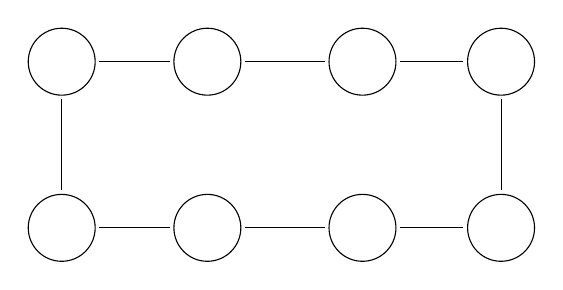
\begin{tikzpicture}[scale=0.5]
				      \draw (11.15, -2.54) circle (0.85);
				      \draw (14.85, -2.54) circle (0.85);
				      \draw (11.15, -6.76) circle (0.85);
				      \draw (14.85, -6.76) circle (0.85);
				      \draw (18.79, -2.54) circle (0.85);
				      \draw (22.31, -2.54) circle (0.85);
				      \draw (18.79, -6.76) circle (0.85);
				      \draw (22.31, -6.76) circle (0.85);
				      \draw (12.11, -2.54) -- (13.89, -2.54);
				      \draw (15.80, -2.54) -- (17.83, -2.54);
				      \draw (19.75, -2.54) -- (21.35, -2.54);
				      \draw (22.31, -3.49) -- (22.31, -5.80);
				      \draw (21.35, -6.76) -- (19.75, -6.76);
				      \draw (17.83, -6.76) -- (15.80, -6.76);
				      \draw (13.89, -6.76) -- (12.11, -6.76);
				      \draw (11.15, -5.80) -- (11.15, -3.49);
			      \end{tikzpicture}
		      \end{center}

	      \end{minipage}%
	      \begin{minipage}[t]{0.45\textwidth}
		      \begin{center}
			      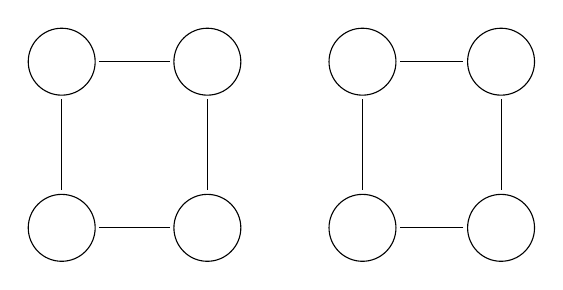
\begin{tikzpicture}[scale=0.5]
				      \draw (11.15, -2.54) circle (0.85);
				      \draw (14.85, -2.54) circle (0.85);
				      \draw (11.15, -6.76) circle (0.85);
				      \draw (14.85, -6.76) circle (0.85);
				      \draw (18.79, -2.54) circle (0.85);
				      \draw (22.31, -2.54) circle (0.85);
				      \draw (18.79, -6.76) circle (0.85);
				      \draw (22.31, -6.76) circle (0.85);
				      \draw (12.11, -2.54) -- (13.89, -2.54);
				      \draw (19.75, -2.54) -- (21.35, -2.54);
				      \draw (22.31, -3.49) -- (22.31, -5.80);
				      \draw (21.35, -6.76) -- (19.75, -6.76);
				      \draw (13.89, -6.76) -- (12.11, -6.76);
				      \draw (11.15, -5.80) -- (11.15, -3.49);
				      \draw (14.85, -3.49) -- (14.85, -5.80);
				      \draw (18.79, -3.49) -- (18.79, -5.80);
			      \end{tikzpicture}
		      \end{center}
	      \end{minipage}
	\item No. Because a graf with $n$ vetexies all with $n-1$ degres is a complete graf, and by definition all complete grafs of degre $n$ are asomorphic
	\item No. Becuase by Handshaking Lemma we have 3 degres of fredom wich is odd number of degref of fredom so the number of verticies shoule be allways even but 5 is odd so is imposible to construc such a graf.
\end{enumerate}

\section*{Problem 6.5}
\begin{enumerate}[label=\arabic*)]
	\item \noindent \\
	      \begin{minipage}{0.5\textwidth}
		      \begin{center}
			      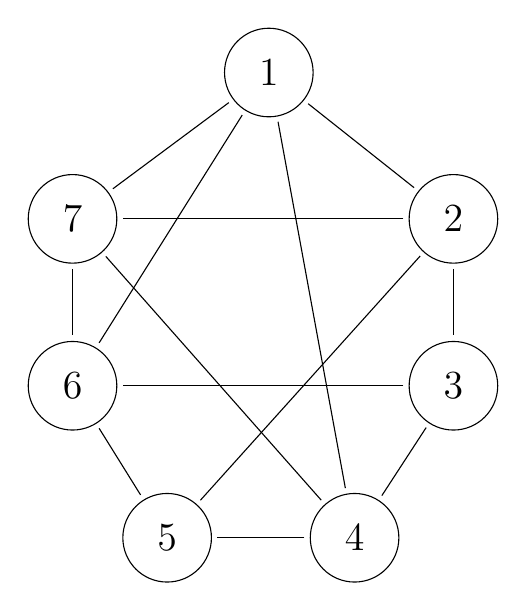
\begin{tikzpicture}[scale=0.45]
				      \draw (29.58, -3.54) circle (1.25);
				      \draw (29.58, -3.54) node {\Large $1$};
				      \draw (24.04, -7.67) circle (1.25);
				      \draw (24.04, -7.67) node {\Large $7$};
				      \draw (34.79, -7.67) circle (1.25);
				      \draw (34.79, -7.67) node {\Large $2$};
				      \draw (24.04, -12.38) circle (1.25);
				      \draw (24.04, -12.38) node {\Large $6$};
				      \draw (34.79, -12.38) circle (1.25);
				      \draw (34.79, -12.38) node {\Large $3$};
				      \draw (26.71, -16.67) circle (1.25);
				      \draw (26.71, -16.67) node {\Large $5$};
				      \draw (32.00, -16.67) circle (1.25);
				      \draw (32.00, -16.67) node {\Large $4$};
				      \draw (30.69, -4.42) -- (33.68, -6.79);
				      \draw (34.79, -9.08) -- (34.79, -10.96);
				      \draw (34.02, -13.56) -- (32.77, -15.48);
				      \draw (30.58, -16.67) -- (28.13, -16.67);
				      \draw (25.96, -15.46) -- (24.79, -13.58);
				      \draw (28.45, -4.39) -- (25.18, -6.82);
				      \draw (24.04, -9.08) -- (24.04, -10.96);
				      \draw (29.84, -4.93) -- (31.74, -15.27);
				      \draw (28.83, -4.74) -- (24.79, -11.17);
				      \draw (33.38, -7.67) -- (25.46, -7.67);
				      \draw (33.85, -8.72) -- (27.65, -15.61);
				      \draw (33.38, -12.38) -- (25.46, -12.38);
				      \draw (31.06, -15.61) -- (24.98, -8.73);
			      \end{tikzpicture}
		      \end{center}
	      \end{minipage}
	      \begin{minipage}{0.5\textwidth}
		      \begin{center}
			      \[a_{ij}=
				      \begin{bmatrix}
					      0 & 1 & 0 & 1 & 0 & 1 & 1 \\
					      1 & 0 & 1 & 0 & 1 & 0 & 1 \\
					      0 & 1 & 0 & 1 & 0 & 1 & 0 \\
					      1 & 0 & 1 & 0 & 1 & 0 & 1 \\
					      0 & 1 & 0 & 1 & 0 & 1 & 0 \\
					      1 & 0 & 1 & 0 & 1 & 0 & 1 \\
					      1 & 1 & 0 & 1 & 0 & 1 & 0
				      \end{bmatrix}\]
		      \end{center}
	      \end{minipage}\\
	      \vspace{1cm}

	      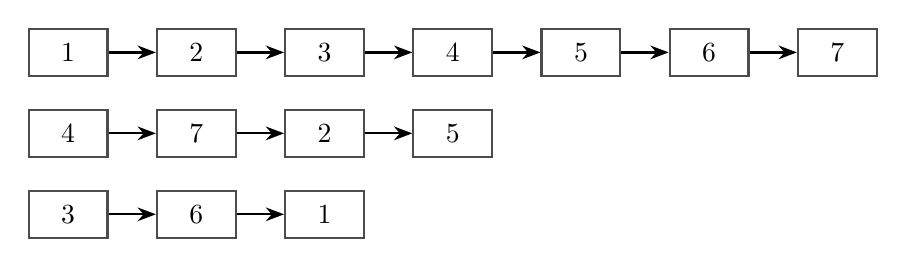
\begin{tikzpicture}[
			      listnode/.style={
					      rectangle,
					      draw=gray!60!black,
					      fill=white!10,
					      thick,
					      minimum width=1cm,
					      minimum height=0.6cm,
					      align=center
				      },
			      >=Stealth,
			      node distance=0.6cm
		      ]

		      % Row 1 -> 2 -> 3 -> 4 -> 5 -> 6 -> 7
		      \node[listnode] (v1) {1};
		      \node[listnode, right=of v1] (v1_1) {2};
		      \node[listnode, right=of v1_1] (v1_2) {3};
		      \node[listnode, right=of v1_2] (v1_3) {4};
		      \node[listnode, right=of v1_3] (v1_4) {5};
		      \node[listnode, right=of v1_4] (v1_5) {6};
		      \node[listnode, right=of v1_5] (v1_6) {7};
		      \draw[->, thick] (v1) -- (v1_1);
		      \draw[->, thick] (v1_1) -- (v1_2);
		      \draw[->, thick] (v1_2) -- (v1_3);
		      \draw[->, thick] (v1_3) -- (v1_4);
		      \draw[->, thick] (v1_4) -- (v1_5);
		      \draw[->, thick] (v1_5) -- (v1_6);

		      % 4 -> 7 -> 2 -> 5
		      \node[listnode, below=0.4cm of v1] (v4) {4};
		      \node[listnode, right=of v4] (v4_7) {7};
		      \node[listnode, right=of v4_7] (v4_2) {2};
		      \node[listnode, right=of v4_2] (v4_5) {5};

		      \draw[->, thick] (v4) -- (v4_7);
		      \draw[->, thick] (v4_7) -- (v4_2);
		      \draw[->, thick] (v4_2) -- (v4_5);

		      % 3 -> 6 -> 1
		      \node[listnode, below=0.4cm of v4] (v3) {3};
		      \node[listnode, right=of v3] (v3_6) {6};
		      \node[listnode, right=of v3_6] (v3_1) {1};

		      \draw[->, thick] (v3) -- (v3_6);
		      \draw[->, thick] (v3_6) -- (v3_1);

	      \end{tikzpicture}
	      \vspace{1cm}
	\item Yes
\end{enumerate}

\section*{Problem 6.6}
The row above we note by $a_i$ the row bellow $b_i$, where the first columns is 1 and the nest to the righ increasing by one
\begin{enumerate}[label=\alph*)]
	\item \textbf{No.} We begin with the most restricitve element \(a_4\) we look the edge \(\{a_4, b_2\}\) because is the only posible edge, but them \(a_2\) can be conected just to \(b_2\) and because we have 2 element that can conect to just one comon element them there does not exist any matchining
	\item \textbf{Yes.} We have \(\{a_2, b_1\},\; \{a_1, b_2\},\; \{a_3, b_3\}\)
	\item \textbf{Yes.} We have \(\{a_2, b_1\},\; \{a_3, b_2\},\; \{a_1, b_3\},\; \{a_4, b_5\},\;\{a_5, b_4\}\)
\end{enumerate}
\newpage
\section*{Problem 6.7}
\begin{enumerate}[label=\alph*)]
	\item From Handshaking lemma, the sum of the degres is the double of the number of edges:
	      \[\sum_{v\in V}{d_G(v)}=2||G||\]
	      \[||G||=\frac{1}{2}\sum_{v\in V}{d_G(v)}\]
	      \[||G||=\frac{1}{2}(2+2+3+4+4+5)=\frac{20}{2}=10\]
	\item 5 faces, we got the from the visual representation of the graf or we could have jut computed them using euler formula \(F=2-V+E=2-6+10=6\) we got 6 faces and we substract 1 from the outerface and we get 5 faces.
	      \vspace{1cm}
	      \begin{center}
		      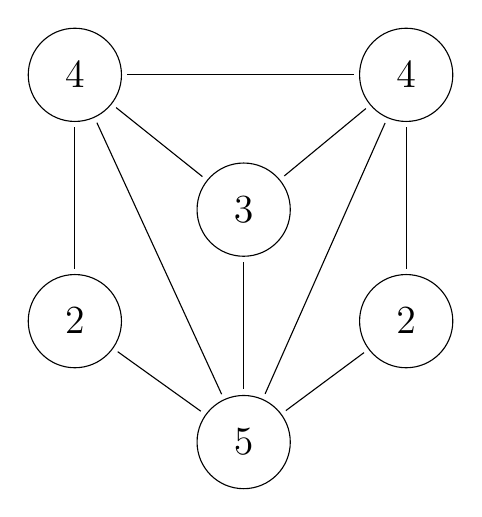
\begin{tikzpicture}[scale=0.4]
			      \draw (28.28, -9.64) circle (1.48);
			      \draw (28.28, -9.64) node {\Large $4$};
			      \draw (38.80, -9.64) circle (1.48);
			      \draw (38.80, -9.64) node {\Large $4$};
			      \draw (33.64, -13.92) circle (1.48);
			      \draw (33.64, -13.92) node {\Large $3$};
			      \draw (33.64, -21.30) circle (1.48);
			      \draw (33.64, -21.30) node {\Large $5$};
			      \draw (28.28, -17.46) circle (1.48);
			      \draw (28.28, -17.46) node {\Large $2$};
			      \draw (38.80, -17.46) circle (1.48);
			      \draw (38.80, -17.46) node {\Large $2$};
			      \draw (29.59, -10.68) -- (32.33, -12.87);
			      \draw (37.52, -10.71) -- (34.93, -12.85);
			      \draw (28.98, -11.16) -- (32.94, -19.78);
			      \draw (38.13, -11.17) -- (34.32, -19.77);
			      \draw (29.64, -18.43) -- (32.28, -20.32);
			      \draw (37.46, -18.46) -- (34.98, -20.30);
			      \draw (38.80, -11.31) -- (38.80, -15.79);
			      \draw (28.28, -11.31) -- (28.28, -15.79);
			      \draw (33.64, -15.59) -- (33.64, -19.62);
			      \draw (29.95, -9.64) -- (37.13, -9.64);
		      \end{tikzpicture}
	      \end{center}
\end{enumerate}

\section*{Problem 6.8}
From euler formula \(V-E+F=1\) so \(6-10+5=1=1\), where $V$ are vertexes, $E$ are edges and $F$ are Faces and. We proved that this is posible expecialy because is the graf in Problem 6.7

\section*{Problem 6.9}
Lest us detone the bipartite graf into two sets $L(G)$ and $R(G)$ and the size of $L$ is $n$ and the sieze of $R$ is $m$. We have the relation $m+n=v$. The maximum number of edges of a bipartite graff is $m \times n$ because we pair each element from $L$ to $R$. We compute the optimal distirbution of vertexes to maximeze the edges.
\[E(n, m)= n\times m\]
\[n+m=e\]
Using Lagrnage multipliers. Or i could have juts rewrote m as \(m=e-n\) and got \(E(n)=n(e-n)\) and computed a derivative but is to boring
\[\nabla E(n, m) = \lambda \nabla(n+m)\]
\[\nabla E(n, m) = (m, n)\]
\[\nabla (n+m) = (1, 1)\]
\[n=\lambda\]
\[m=\lambda\]
\[n=m\]
\[n+n=e\]
\[n=e/2\]
\[E_{max}=\frac{e^2}{4}\]
But this is a planar graf, so what i did so far is wrong,
\section*{Problem 6.10}
\begin{enumerate}[label=\alph*)]
	\item It does not hold. But if we treat the as $n$ grafs with more that 1 vertex each Euler formulas works on each one of them individualy and we coudl write this as \[\sum^n_i(v_i-e_1+f_i)=n+1\] but if at leas one is disconected it does not work. It work because we can aplie euler formula to each individual component but when we sum the we add $n$ times the external face so we substract $n$ to get the internal faces, and add one to take into acout the exeternal one just once.
	\item We do the same thing as at a), but we treat the conected component as a component and we get \[\sum^(n-1)_i(v_i-e_1+f_i)=(n-1)+1=n\]
	\item We generalize b and get \[\sum^(n-k)_i(v_i-e_1+f_i)=(n-k)+1\]. and for the case \(k=n-1\) it reduces to $v-e+f=2$
\end{enumerate}

\section*{Problem 6.11}
By the 4 colour theorem as planar graff can be colored by at most 4 colors so if a graf has a chromatic number bigger that 4 wich is in our case 6 is biger than 4 this means that it cann't be a planar graff

\section*{Problem 6.12}
Just 1. Because to have a Euler circuit there should exist a maximum of 0 or 2 vertexes with a even but we have 4 verticies the central iled habing a degre 5, and other a degre 3 and the 2 part of the city a degre 3, and if we add just a brige betwen the iland A and iland D they will have degres 6 and 4 wich by euler will alow us to make a euler trail.


\section*{Problem 6.13}
Just 1. Because to have a Euler circuit there should exist a maximum of 0 or 2 vertexes with a even but we have 4 verticies the central iled habing a degre 5, and other a degre 3 and the 2 part of the city a degre 3, and if we add just a brige betwen the iland A and iland D they will have degres 6 and 4 wich by euler will alow us to make a euler trail.

\section*{Problem 6.14}
\begin{enumerate}[label=\alph*)]
	\item Yes because by Euler circuit we have 2 vertexis of odd degre(3 and 6) the rest being even, wich allows us to constru a Eulean trail, the condition being that we begin at one of the rooms with an odd number of dors
	      \begin{figure}[H]
		      \centering
		      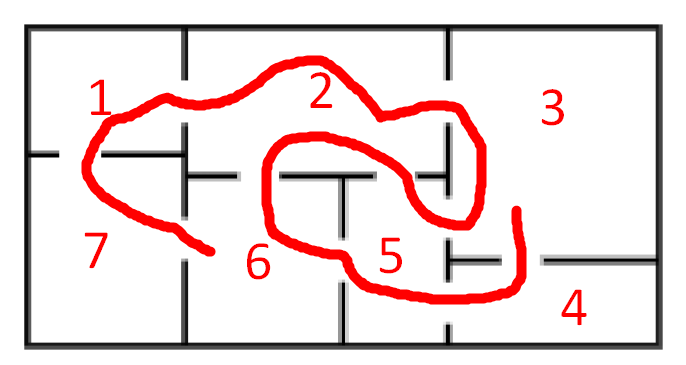
\includegraphics[width=0.7\textwidth]{image.png}
	      \end{figure}
	\item Yes, because we can represent the house as a planar graff.
	      \begin{figure}[H]
		      \centering
		      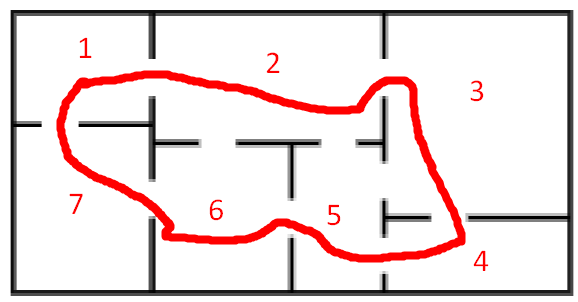
\includegraphics[width=0.7\textwidth]{Screenshot_1.png}
	      \end{figure}
	\item Yes. From the Handshaking lemma
	      \[\sum_{v \ in V}d_G(v) = 2||G||\]
	      we can write each room degre as $d_G(v)=2a_i+1$
	      \[\sum_{v \ in V}d_G(v) = \sum^6_{i}(2a_i+1)=\sum^6_{i}{2a_i}+\sum^6_{i}{1}=2\sum^6_{i}+6\]
	      We know that $\displaystyle 2\sum^6_{i}$ is allways even and 6 is even and even+even = even number and becose $2||G||$ is olso always even wich means is posible for all roms to have a odd number of doors
\end{enumerate}

\section*{Problem 6.15}
We begin with the most restricitve element, the triangle $T_1, T_2, T_3 $ we die them yellow, blue and red respectivly, and them i die \(T_4\) either yellow or red, but i chose red, and now we die \(T_5\) blue and that it, cromatic number 3.
\begin{center}
	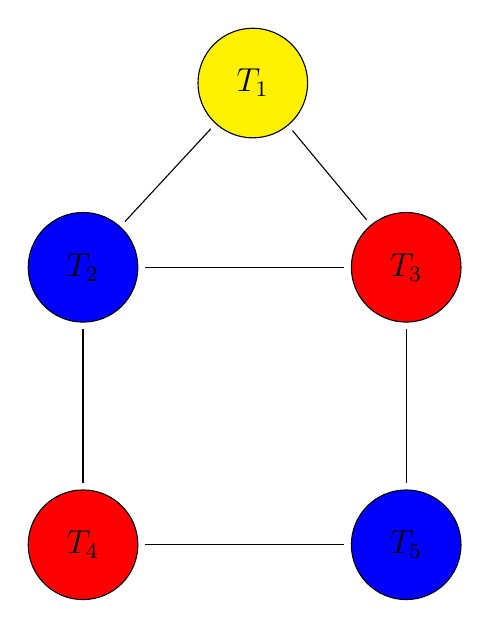
\begin{tikzpicture}[scale=0.4]
		\filldraw[fill=yellow] (39.71, -12.70) circle (1.74);
		\draw (39.71, -12.70) node {\large $T_1$};
		\filldraw[fill=blue] (34.32, -18.55) circle (1.74);
		\draw (34.32, -18.55) node {\large $T_2$};
		\filldraw[fill=red] (44.58, -18.55) circle (1.74);
		\draw (44.58, -18.55) node {\large $T_3$};
		\filldraw[fill=red] (34.32, -27.36) circle (1.74);
		\draw (34.32, -27.36) node {\large $T_4$};
		\filldraw[fill=blue] (44.58, -27.36) circle (1.74);
		\draw (44.58, -27.36) node {\large $T_5$};
		\draw (38.38, -14.15) -- (35.65, -17.10);
		\draw (40.97, -14.21) -- (43.32, -17.04);
		\draw (36.29, -18.55) -- (42.61, -18.55);
		\draw (34.32, -20.52) -- (34.32, -25.39);
		\draw (36.29, -27.36) -- (42.61, -27.36);
		\draw (44.58, -20.52) -- (44.58, -25.39);
	\end{tikzpicture}
\end{center}


\section*{Problem 6.16}
\begin{enumerate}[label=\alph*)]
	\item By the Handshaking lemma we have \(\sum_{v\in V}d_G(v)=2||G||\) so we have \[ ||G||=\frac{4 \times 3 + (n-4)}{2} = \frac{n}{2}+4\]
	      \[||G||=n-1\]
	      \[n-1=\frac{n}{2}+4\]
	      \[2n-2=n+8\]
	      \[n=10\]
\begin{center}
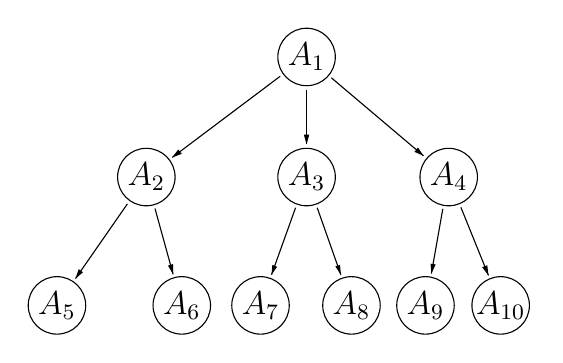
\begin{tikzpicture}[scale=0.5]
\draw (17.66, -4.49) circle (0.73);
\draw (17.66, -4.49) node {\large $A_1$};
\draw (13.59, -7.54) circle (0.73);
\draw (13.59, -7.54) node {\large $A_2$};
\draw (17.66, -7.54) circle (0.73);
\draw (17.66, -7.54) node {\large $A_3$};
\draw (21.27, -7.54) circle (0.73);
\draw (21.27, -7.54) node {\large $A_4$};
\draw (11.32, -10.80) circle (0.73);
\draw (11.32, -10.80) node {\large $A_5$};
\draw (14.49, -10.80) circle (0.73);
\draw (14.49, -10.80) node {\large $A_6$};
\draw (16.49, -10.80) circle (0.73);
\draw (16.49, -10.80) node {\large $A_7$};
\draw (18.80, -10.80) circle (0.73);
\draw (18.80, -10.80) node {\large $A_8$};
\draw (22.59, -10.80) circle (0.73);
\draw (22.59, -10.80) node {\large $A_{10}$};
\draw (20.68, -10.80) circle (0.73);
\draw (20.68, -10.80) node {\large $A_9$};
\draw (16.99, -4.98) -- (14.25, -7.04);
\fill (14.40,-6.84) -- (14.49,-6.95) -- (14.25,-7.04) -- cycle;
\draw (17.66, -5.32) -- (17.66, -6.71);
\fill (17.59,-6.46) -- (17.73,-6.46) -- (17.66,-6.71) -- cycle;
\draw (18.29, -5.02) -- (20.63, -7.00);
\fill (20.40,-6.90) -- (20.49,-6.79) -- (20.63,-7.00) -- cycle;
\draw (13.11, -8.22) -- (11.79, -10.12);
\fill (11.87,-9.88) -- (11.98,-9.96) -- (11.79,-10.12) -- cycle;
\draw (13.81, -8.34) -- (14.27, -10.01);
\fill (14.14,-9.79) -- (14.27,-9.75) -- (14.27,-10.01) -- cycle;
\draw (17.38, -8.32) -- (16.77, -10.02);
\fill (16.79,-9.77) -- (16.91,-9.82) -- (16.77,-10.02) -- cycle;
\draw (17.93, -8.32) -- (18.53, -10.02);
\fill (18.39,-9.81) -- (18.51,-9.77) -- (18.53,-10.02) -- cycle;
\draw (21.12, -8.35) -- (20.83, -9.99);
\fill (20.81,-9.74) -- (20.94,-9.76) -- (20.83,-9.99) -- cycle;
\draw (21.58, -8.31) -- (22.28, -10.04);
\fill (22.12,-9.83) -- (22.25,-9.78) -- (22.28,-10.04) -- cycle;
\end{tikzpicture}
\end{center}
\item  The longest path with the property that we do not go over the same element twice in the first graf is os size 5, an example would be \(A_5 \rightarrow A_2 \rightarrow A_1 \rightarrow A_4 \rightarrow A_{10}\)  but in the second one example is \(B_1 \rightarrow B_2 \rightarrow B_3 \rightarrow B_5 \rightarrow B_7 \rightarrow B_9\) wich is os size 6 and is imposible to create a bijection betwen this 2 pafs so the grafs are not isomorphic \noindent \vspace{1cm}
\begin{center}
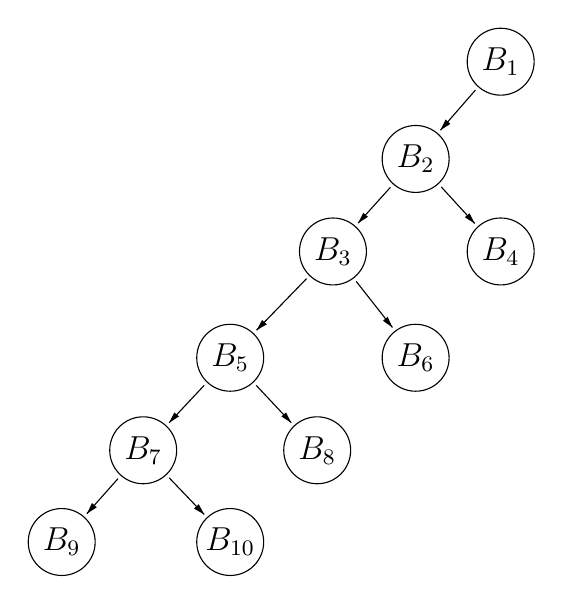
\begin{tikzpicture}[scale=0.5]
\draw (18.27, -3.38) circle (0.85);
\draw (18.27, -3.38) node {\large $B_2$};
\draw (16.17, -5.73) circle (0.85);
\draw (16.17, -5.73) node {\large $B_3$};
\draw (20.43, -5.73) circle (0.85);
\draw (20.43, -5.73) node {\large $B_4$};
\draw (13.56, -8.43) circle (0.85);
\draw (13.56, -8.43) node {\large $B_5$};
\draw (18.27, -8.43) circle (0.85);
\draw (18.27, -8.43) node {\large $B_6$};
\draw (11.35, -10.78) circle (0.85);
\draw (11.35, -10.78) node {\large $B_7$};
\draw (15.77, -10.78) circle (0.85);
\draw (15.77, -10.78) node {\large $B_8$};
\draw (9.28, -13.11) circle (0.85);
\draw (9.28, -13.11) node {\large $B_9$};
\draw (13.56, -13.11) circle (0.85);
\draw (13.56, -13.11) node {\large $B_{10}$};
\draw (20.43, -0.91) circle (0.85);
\draw (20.43, -0.91) node {\large $B_1$};
\draw (17.63, -4.10) -- (16.81, -5.01);
\fill (16.94,-4.75) -- (17.06,-4.85) -- (16.81,-5.01) -- cycle;
\draw (18.92, -4.09) -- (19.77, -5.02);
\fill (19.52,-4.86) -- (19.64,-4.76) -- (19.77,-5.02) -- cycle;
\draw (15.50, -6.42) -- (14.23, -7.73);
\fill (14.37,-7.47) -- (14.49,-7.58) -- (14.23,-7.73) -- cycle;
\draw (16.76, -6.49) -- (17.68, -7.66);
\fill (17.44,-7.49) -- (17.56,-7.39) -- (17.68,-7.66) -- cycle;
\draw (12.90, -9.13) -- (12.01, -10.08);
\fill (12.14,-9.82) -- (12.26,-9.92) -- (12.01,-10.08) -- cycle;
\draw (14.22, -9.13) -- (15.11, -10.08);
\fill (14.86,-9.92) -- (14.98,-9.82) -- (15.11,-10.08) -- cycle;
\draw (10.71, -11.50) -- (9.92, -12.39);
\fill (10.05,-12.12) -- (10.17,-12.23) -- (9.92,-12.39) -- cycle;
\draw (12.01, -11.48) -- (12.90, -12.41);
\fill (12.64,-12.26) -- (12.76,-12.15) -- (12.90,-12.41) -- cycle;
\draw (19.79, -1.63) -- (18.90, -2.65);
\fill (19.03,-2.38) -- (19.15,-2.49) -- (18.90,-2.65) -- cycle;
\end{tikzpicture}
\end{center}
\end{enumerate}

\section*{Problem 6.17}
We know that
\[\Delta (T) = \max_{v \in V}\{d_T(v)\}\]
and olso we define the number of leafs as $N(T) = n$.
\begin{proof} \noindent \\
Base Cases:
\begin{enumerate}[label=\arabic*)]
	\item $N(T)=1$, them $\Delta(T) =0$ and $1>0$
	\item $N(T)=2$, them $\Delta(T) =1$ and $2>1$
\end{enumerate}
Inductive Step
By the handsake lemma we have \(\sum_{v\in V}d_T(v)=2||T||\) and we know that $||T||=n-1$ so $$2(n-1)=\sum_{v\in V}d_T(v)$$
$$2n-2=\sum_{v\in V}d_T(v) \le \max{d_T(v)}$$
$$2n-2 > 2n > n \implies n < \sum_{v\in V}d_T(v) \le \max{d_T}$$
\end{proof}



\section*{Problem 6.18}
\begin{proof} \noindent \\
By $n$  we define the number of vertexes and $E(t)$ we define the number of edges
Base Cases:
\begin{enumerate}[label=\arabic*)]
	\item $n=0$, $E(T)=0$ trivial!
	\item $n=1$, $E(T)=1-1=0$
	\item $n=2$, $E(T)=2-1=1$
\end{enumerate}
Inductive Step
$N(n)=n-1$ if we add another edge we get $N(n+1)=n+1$ hovewer because the graf is acyclical and conected we shoudl conect those 2 vertexis by one edge so $E(n+1)=E(n)+1$
$E(n+1)=n+1-1=n$ and we know that $E(n+1)=E(n)+1=(n-1)+1=n$ and $n=n$ so we proved that the formula holds
\end{proof}



\end{document}